\label{gaps} 

It is indisputable that many phonotactic restrictions are easily described with reference to prosodic primitives.
In some cases, prosodic factors constrain the system of contrast.
For instance, Latin has contrastive vowel and consonant length (e.g., \emph{os} `bone' vs.~\emph{ōs} `mouth', \emph{anus} `ring' vs.~\emph{annus} `year'), but the latter contrast is suspended in codas preceded by a diphthong or long monophthong; a syllable may contain a long vowel, or be checked by the first half a geminate consonant, but not both.
However, constraints on underlying representations may also involve references to non-contrastive prosodic structures such as the syllable (e.g., \citealt{Hooper1973}, \citealt{Kahn1976}).\footnote{
    See \citealt{Blevins1995} for the claim that syllable structure is universally non-contrastive, and \citealt{Elfner2006} for arguments that a putative counterexample derives from an underlying vowel length contrast.}
For instance, as noted by \citet{Haugen1956}, 
numerous restrictions on word-medial consonant clusters have a unified statement in prosodic terms:

\begin{example}[\textsc{Medial Cluster Law}]
\label{mcl}
A medial cluster can consist maximally of a well-formed medial coda and a well-formed medial onset
\end{example}

As an illustration of this tautology, consider languages like Yokuts, which forbid complex codas and complex onsets, and which enforce these restrictions in complex words via processes such as vowel epenthesis.
\citet[26f.]{Newman1944} notes that this imposes an an upper bound on the size of medial clusters: no cluster of more than two consonants can be parsed into a simple coda and simple onset.
In the case of Yokuts, it is certainly possible to state this restriction without reference to syllable structure, as *CCC, a constraint on trisyllabic clusters (e.g., \citealt[92f.]{Ettlinger2008}, \citealt[820f.]{Zuraw2003a}).
However, the aforementioned constraints on complex onsets and codas find independent motivation from the total absence of initial and final clusters in Yokuts;\footnote{
    The tendency of consonants to pattern with word boundaries and morph junctures has been long been noted \citep[e.g.,][]{Hill1954,Lass1971,Moulton1947}; \citet[24f.]{Kahn1976} takes this as evidence for the syllable.}
with these two restrictions in place, a further constraint on medial triconsonantal clusters is otiose.\footnote{
    \citet[31f.]{Cote2000} alludes to another critique of constraints like *CCC, namely that this constraint requires ``counting'': see \citealt[64f.]{Isac2008} for further discussion of the comparative merits of ``counting'' and ``grouping'' analyses in phonology.}
While the medial cluster law is certainly consistent with the hypothesis that syllable structure may be present in underlying representations (e.g., \citealt{A74}:255, \citealt{Vaux2003}), this need not be the case under Stampean occultation.
If an underlying medial consonant sequence appears on the surface, it satisfies the medial cluster law by definition.
If, however, an underlying cluster is modified by consonant deletion, coalescence, or vowel epenthesis, then it need not consist of a licit medial onset and medial coda.

\citet{Pierrehumbert1994} begins a study of English word-medial consonant clusters with a restatement of the medial cluster law:

\begin{quote}
That is, in the absence of additional provisos, any concatenation of a well-formed coda and a well-formed onset is predicted to be possible medially in a word. \citep[168]{Pierrehumbert1994}
\end{quote}

\noindent
However, \citeauthor{Pierrehumbert1994} reports that the vast majority of the ``possible'' clusters (i.e., those which conform to the medial cluster law) are in fact unattested. 
So as to acount for this, \citeauthor{Pierrehumbert1994} presents ``provisos'' in the forms of static co-occurrence restrictions, unrelated to any phonological alternation in English.\footnote{
    Given the arguments presented in the previous chapter, that not all lexical tendencies have a synchronic basis, one may question the intuition that any gaps in the English cluster inventory (or those that go beyond the medial cluster law) must be accounted for by the synchronic grammar.
    In addition to some informal statistical evidence (of the sort problematized in the previous chapter), \citeauthor{Pierrehumbert1994} administers a wordlikeness task to validate the static constraints she proposes.
    However, this experiment is of a quite informal nature and the results are given only a superficial analysis, so it is less than probative.} 
This chapter will argue, however, the static constraints proposed by \citeauthor{Pierrehumbert1994} are unnecessary, and that the only restrictions on the inventory of medial clusters in English (beyond the medial cluster law) are those which derive from well-known phonological processes.

\section{English syllable contact clusters}

The aforementioned study by \citeauthor{Pierrehumbert1994}, as well as further investigations of this domain by \citet[ chap.~8]{Duanmu2009} and \citet[ chap.~3]{Hammond1999a}, argue for the necessity of admitting static phonotactic constraints, and illustrate proposals for the architecture of the phonotactic system.
However, there are a number of reasons to reconsider the findings of these authors in light of the proposals made in previous chapters.

\subsection{The role of phonological processes}

\citeauthor{Duanmu2009}, \citeauthor{Hammond1999a}, and \citeauthor{Pierrehumbert1994} do not generally take into account the effects of phonological processes which target medial clusters in English.
As a consequence, some of the static constraints these authors identify may be in fact the product of English morphophonemics and Stampean occultation. 
For instance, \citeauthor{Pierrehumbert1994} writes that ``nasal-stop sequences agree in labiality'' (175) and posits a static constraint to account for this fact.
However, this generalization is merely a narrower form of a restriction deriving from a process of \textsc{Nasal Place Assimilation} (see \S\ref{npa}).
Other derived constraints are simply not mentioned; for instance, \citeauthor{Pierrehumbert1994} does not discuss the highly reliable tendency of obstruent-obstruent clusters to agree in voicing (see \S\ref{ova}); while \citet{Hammond1999a} does allude to this restriction, it is dismissed in light of a few apparent counterexamples (though see \S\ref{sss:map} below).
In contrast, this chapter attempts to evaluate derived and static constraints on an equal footing.

\subsection{The role of sparsity}

\citet{Pierrehumbert1994} infers static constraints from near-exceptionless gaps in the lexicon, but little effort is made to show that the patterns of lexical underrepresentation are not due to chance. 
Consequently, it is possible to suggest that some of these gaps are accidental rather than structural in nature.
This is made all the more likely given the tendency of segment and cluster frequency distributions to be highly skewed \citep[e.g.,][]{Pande2010,Sigurd1968,Tambovtsev2007,Weiss1961} so that it is difficult to distinguish between structural and accidental gaps.
Furthermore, \citeauthor{Pierrehumbert1994} considers only triconsonantal clusters, but medial clusters may be as short as two consonants, as in \emph{a}[n.t]\emph{ics}, or as long as four, as in \emph{mi}[n.str]\emph{el}, and no justification is given for ignoring clusters of other lengths.
If there is any effect of this focus, it is presumably to produce further sparsity in the distribution observed.

\subsection{The role of morphological segmentation}

Many components of \citeauthor{Pierrehumbert1994}'s study cannot be replicated.
\citeauthor{Pierrehumbert1994} limits her study to words she judges to be ``morphologically simple'' and ``reasonably familiar''; the author's sensations thereof are not replicable, nor are they available to other researchers in any form.
It has been suggested \citep[e.g.,][]{Labov1975,Schutze1996} that the sensations (as well as cognitive limitations) of concerned parties should not be granted evidential status in the first place, given the potential for implicit bias; \citeauthor{Labov1975} calls the \emph{Experimenter Principle}.

It is not uncommon for analysts to propose otherwise-unmotivated morphological junctures simply to preserve phonological or phonotactic generalizations.
This is done by \citet{SPE}, for instance, to simplify principles of English stress assignment.
Similarly, \citet[546]{Rice2009d} analyses many words in Slave as compounds simply because they contain consonant clusters that rarely occur in morph-internal contexts.
%There is some evidence that infants \citep{Mattys2001b} and adults \citep{Brown1956,Hay2004a,McQueen1998b,Norris1997} use this heuristic to segment fluent speech in experimental settings.
Applied indiscriminately, however, this heuristic trivializes both morphological segmentation and phonotactic generalization.
For these reasons, the wordlist used in this study is derived from a publicly available database, and no experimenter intuitions are used.

\section{Evaluation}
\label{4evaluation}

After constructing a sample of syllable contact clusters in English simplex words, this sample is used to evaluate the coverage of static and derived constraints.

\subsection{Method}

\subsubsection{Materials and procedure}
\label{sss:map}

Following \citet[ chap.~8]{Duanmu2009} and \citet[ chap.~3]{Hammond1999a}, who also consider restrictions on English medial clusters, a wordlist is generated using the English portion of the CELEX database \citep{CELEX}.
Only words marked in CELEX as ``monomorphemic'' are used, and all words labeled in CELEX as non-native are excluded.\footnote{
    The first criterion results in the exclusion of proper names, which have long been noted to push the bounds of native language phonotactics \citep[e.g.,][254]{Trubetzkoy1939}.}
These more-stringent criteria exclude many words labeled exceptions in the studies by \citeauthor{Duanmu2009} or \citeauthor{Hammond1999a} in their studies.
For instance, nearly all the exceptions to \textsc{Obstruent Voice Assimilation} (see \S\ref{ova} below) noted by \citet[74]{Hammond1999a} are excluded either as complex words (e.g., \emph{jurisdiction}, \emph{madcap}, \emph{tadpole}, \emph{scapegoat}, \emph{magpie}) or non-native (e.g., \emph{vodka}, \emph{smorgasbord}).

In contrast to prior studies, these criteria also exclude words which consist of a Latinate prefix and a bound stem (e.g., \emph{inspect}, \emph{excrete}). 
While \citeauthor{Pierrehumbert1994} rejects this analysis as as unmotcontroversial, it in fact has extensive formal and experimental support.
First, Latinate prefixes simplify the statement of many morphophonemic details in English.
For instance, \citet[11f.]{Aronoff1976} observes that Latinate forms which share the same bound stem also share irregular allomorphs of that stem under derivation. 

\begin{example}[Bound stem-specific allomorphy]
\begin{tabular}{l l l l l l}
a. & {adhere}   & {adhesion}   \\
   & {cohere}   & {cohesion}   \\
b. & {conceive} & {conception} \\
   & {perceive} & {perception} \\
\end{tabular}
\end{example}

\noindent
\citeauthor{Aronoff1976} takes this to be evidence that \emph{adhere} and \emph{cohere}, for instance, share a bound stem.
There is also an interaction between Latinate prefixes on verbs and the complements they select.
Latinate verbs do not generally allow ditransitive, verb participle, or adjectival resultative constructions, all of which are acceptable with similar Anglo-Saxon verbs \citep[e.g.,][]{Gropen1989,Harley2009}.

\begin{example}[Restrictions on Latinate verbal complements]
\label{harley}
\begin{tabular}{l l l l@{} l}
a. & {show him the painting} & \alt{} & * & {exhibit him the painting} \\
b. & {drink himself stupid}  & \alt{} & * & {imbibe himself stupid}    \\
c. & {break it off}          & \alt{} & * & {terminate it off}         \\
\end{tabular}
\end{example}

Lexical decision also provide evidence for the segmentation of Latinate prefixed forms.
\citet{Taft1975,Taft1976} and \citet{Taft1986} find that nonce words like \emph{*re-sert}, which appear to be composed of a prefix and a bound stem, take longer to reject that non-words which lack apparent morphological structure, such as *\emph{refant}. 
Bound stems also show frequency effects independent of whole word frequency \citep{Taft1979,Taft2006}.
Finally, \citet{Emmorey1989} and \citet{Forster2000} report facilitative priming, thought to implicating morphological relatedness, between pairs like \emph{permit}-\emph{submit}, which appear to share a bound stem.

\subsection{Results}

Filtering the CELEX data according to the above criteria results in a list of 6,619 simplex words.
The full set of clusters and their frequencies are listed in Appendix \ref{clusters}.
The CELEX transcriptions of these words are then syllabified and phonologized using a procedure
%the same procedure as used in Chapter \ref{gradience} and
described in Appendix \ref{syllabification}. 
In all, the sample contains 23 different medial coda and 40 different medial onsets.
Of the 920 ($= 21 \times 40$) medial clusters that would result from free combination of medial coda and medial onset, 174 (19\%) are attested.

\subsubsection{Static constraints}

To account for the 81\% of ``possible'' but unattested clusters, \citet{Pierrehumbert1994} proposes three static constraints on English medial clusters.

\paragraph{Dorsal-labial clusters}
\citet[173]{Pierrehumbert1994} writes that ``velar obstruents occurred only before coronals in the clusters studied, never before labials or other velars'', while noting that absence of velar-velar clusters is expected due to a separate constraint on geminate clusters (see \S\ref{degemx}).
However, biliteral velar-labial clusters are found in words such as \emph{a}[k.m]\emph{e}, \emph{ru}[ɡ.b]\emph{y}, or \emph{pi}[ɡ.m]\emph{ent}.
Velar-labial clusters are somewhat less common than velar-coronal clusters (e.g., \emph{ve}[k.t]\emph{or}), but such underrepresentation is not unlikely to occur by chance according to the Fisher exact test (Table \ref{dltab}).

\begin{table}
\centering
\begin{tabular}{l rrrr}
\toprule
           & attested & unattested & saturation & $p$-value \\
\midrule
conforming & 25       & 91         & 22\%       & \multirow{2}{*}{.106} \\
violating  &  4       & 40         &  9\%       \\
\bottomrule
\end{tabular}
\caption{Dorsal-labial cluster attestation in the lexical sample}
\label{dltab}
\end{table}

\paragraph{Coronal obstruent codas}
\citet[175]{Pierrehumbert1994} claims that ``clusters with a coronal obstruent in the coda do not occur'', but at the same time observes exceptions like \emph{a}[nt.l]\emph{er}, \emph{ke}[s.tr]\emph{el} and \emph{oi}[nt.m]\emph{ent}.
In the CELEX sample (Table \ref{cctab}), coda coronal obstruent clusters are not significantly less likely to occur than non-coronal obstruent clusters (e.g., \emph{re}[p.t]\emph{ile}).
While not shown in tabular form, the same is true if attention is restricted to triconsonantal clusters ($p = .129$).

\begin{table}
\centering
\begin{tabular}{l rrrr}
\toprule
           & attested & unattested & saturation & $p$-value \\
\midrule
conforming & 56       & 304        & 15\%       & \multirow{2}{*}{.430} \\
violating  & 37       & 243        & 13\%       \\
\bottomrule
\end{tabular}
\caption{Coda coronal obstruent cluster attestation in the lexical sample}
\label{cctab}
\end{table}

\paragraph{ABA clusters} 
\citet[176]{Pierrehumbert1994} observes a ``lack of clusters with identical first and third elements'', ignoring presence or absence of voicing. 
Despite the fact that there are no exceptions to this generalization, these \textsc{ABA} clusters are not significantly less common than any other triconsonantal and quadraconsonantal clusters (Table \ref{abatab}).

\begin{table}
\centering
\begin{tabular}{l rrrr}
\toprule
           & attested & unattested & saturation & $p$-value \\
\midrule
conforming & 47       & 512        &  8\%       & \multirow{2}{*}{.250} \\
violating  &  0       &  25        &  0\%       \\
\bottomrule
\end{tabular}
\caption{ABA cluster attestation in the lexical sample}
\label{abatab}
\end{table}

\paragraph{Summary} 
There is no statistical support for any of \citeauthor{Pierrehumbert1994}'s static constraints.

\subsubsection{Derived constraints}

In \emph{SPE}, \citet{SPE} describe three phonological processes which target medial consonant clusters. 
As will be shown, these three processes have a profound influence on the English cluster inventory.

\paragraph{Obstruent voice assimilation}
\label{ova}

Voice assimilation alternations are evidenced by the non-syllabic allomorphs of the regular past (e.g., \emph{nap}[t]-\emph{nab}[d]) and noun plural (e.g., \emph{lap}[s]-\emph{lab}[z]), which take the voicing specification of a preceding obstruent;\footnote{
    Underlying /-d, -z/ are assumed here (e.g., \citealt{Anderson1973a}, \citealt[284f.]{Bakovic2005b}, \citealt{Basboll1972}, \citealt[210]{SPE}, \citealt[282]{Hockett1958}, \citealt[102]{Pinker1988}, \citealt{Shibatani1972}); alternative analyses are put forth by \citet[210f.]{LANGUAGE}, \citet[135]{Borowsky1986}, \citet{Hoard1971}, \citet{Kiparsky1985}, \citet{Lightner1970}, \citet{Luelsdorff1969}, \citet{Miner1975}, \citet[426]{Nida1948}, and \citet{Zwicky1975}.} 
voice assimilation is also claimed to operate across prefix and compound junctures \citep{Davidsen-Nielsen1974}.
%Bizarely, \citet[208]{Wetzels2001}, cite English as an example of a language without ``general devoicing or assimilatory effects''. 

\begin{example}[\textsc{Obstruent Voice Assimilation}]
\label{ovarule}
$\begin{bmatrix} -\textsc{Son} \end{bmatrix}~\goesto~\begin{bmatrix} =\textsc{Voi} \end{bmatrix}~/~\gap~\begin{bmatrix} =\textsc{Voi} \\ -\textsc{Son} \end{bmatrix}$
\end{example}

\noindent
\citet{Pierrehumbert1994} does not discuss a constraint against adjacent obstruents disagreeing in voice. 
However, the vast majority of medial obstruents clusters in simplex words are either uniformly voiced, as in \emph{hu}[z.b]\emph{and}, or uniformly voiceless, as in or \emph{rha}[p.s]\emph{osdy} (Table \ref{ovatab}).
Hetero-voiced clusters, like those in \emph{a}[b.s]\emph{inth} and \emph{a}[s.b]\emph{estos}, are far rarer than would be expected from chance.

\begin{table}
\centering
\begin{tabular}{l rrrr}
\toprule
           & attested & unattested & saturation & $p$-value \\
\midrule
conforming & 35       & 329        & 10\%       & \multirow{2}{*}{.002} \\
violating  & 11       & 305        &  3\%       \\
\bottomrule
\end{tabular}
\caption{Obstruent voice assimilation cluster attestation in the lexical sample}
\label{ovatab}
\end{table}

\paragraph{Nasal place assimilation}
\label{npa}

\textsc{Nasal Place Assimilation} (e.g., \citealt[65f.]{Borowsky1986}, \emph{SPE}:85, \citealt[62]{Halle1985a})
%\citealt[269]{Fudge1969})
permits [ŋ] to be described as an allophone of /n/ (see \S\ref{s:phonologization}), and furthermore accounts for allomorphy in certain Latinate prefixes.

\begin{example}[\emph{im-}/\emph{in-} allomorphy]
\label{nparule}
\begin{tabular}{l l l l l l l}
a. & {polite}   & {i}[m.p]{olite}   \\
   & {balance}  & {i}[m.b]{alance}  \\
b. & {tangible} & {i}[n.t]{angible} \\
   & {decent}   & {i}[n.d]{ecent}   \\
\end{tabular}
\end{example}

%Furthermore, \citet[228]{Myers1993} reports speech errors which create nasal-obstruent clusters and undergo \textsc{Nasal Place Assimilation}; e.g., \emph{ra}[nd] \emph{orker}, intended \emph{ra}[ŋk] \emph{order}. 

\noindent
The rule is formalized below.

\begin{example}[\textsc{Nasal Place Assimilation}]
$\begin{bmatrix} $+$\textsc{Nas} \end{bmatrix}~\goesto~\begin{bmatrix} =\textsc{Lab} \\ =\textsc{Cor} \\ =\textsc{Dor} \end{bmatrix}~/~\gap{}~\begin{bmatrix} =\textsc{Lab} \\ =\textsc{Cor} \\ =\textsc{Dor} \\ -\textsc{Son} \end{bmatrix}$
\end{example}

\noindent
Virtually all clusters consisting of a nasal coda followed by a homorganic obstruent (e.g., \emph{pi}[m.p]\emph{le}, \emph{sta}[n.z]\emph{a}, \emph{mo}[ŋ.k]\emph{ey}) are attested (Table \ref{npatab}).
As \citet[175]{Pierrehumbert1994} observes, heterorganic clusters, like those \emph{pli}[m.s]\emph{oll} or \emph{scri}[m.ʃ]\emph{aw}, do occur, but in this sample they are significantly more rare.

\begin{table}
\centering
\begin{tabular}{l rrrr}
\toprule
           & attested & unattested & saturation & $p$-value \\
\midrule
conforming & 31       & 2          & 94\%       & \multirow{2}{*}{3.4\e{-07}} \\
violating  & 11       & 22         & 33\%       \\
\bottomrule
\end{tabular}
\caption{Nasal place assimilation cluster attestation in the lexical sample}
\label{npatab}
\end{table}

\paragraph{Degemination}
The final alternation found in English medial clusters is the simplification of geminates which is characteristic of ``level I'' morphology, and is found in the irregular /-t/ past tense (e.g., \emph{bend}/\emph{ben}[t], \emph{build}/\emph{buil}[t]), in \emph{-ly} deadjectival derivatives (e.g., \emph{norma}[l]\emph{y}, cf.~\emph{calm}[l]\emph{y}), and Latinate prefix allomorphy (\citealt[102]{Borowsky1986}, \emph{SPE}:148).
\textsc{Degemination} is formalized here as a rule deleting the first of two segments agreeing on all feature values (except for voice, possibly).
\label{degemx}

\begin{example}[\textsc{Degemination}]
$\begin{bmatrix} =\textsc{Lab} \\ =\textsc{Cor} \\ =\textsc{Dor} \\ =\textsc{Son} \\ \ldots{} \end{bmatrix}~\goesto~\emptyset~\big /~\gap~\begin{bmatrix} =\textsc{Lab} \\ =\textsc{Cor} \\ =\textsc{Dor} \\ =\textsc{Son} \\ \ldots{} \end{bmatrix}$
\end{example}

\noindent
The sample contains no sequences of identical segments, or of identical segments differing only in voice, something highly unlikely to arise by chance (Table \ref{degemtab}); \textsc{Degemination} and Stampean occultation provide a natural explanation for this gap.
It is interesting to compare the absense of geminates to the constraint against ``ABA'' clusters proposed by \citeauthor{Pierrehumbert1994} in this regardl: both are exceptionless, but only the former imposes a lexical tendency unlikely to arise by chance.

\begin{table}
\centering
\begin{tabular}{l rrrr}
\toprule
           & attested & unattested & saturation & $p$-value \\
\midrule
conforming & 173      & 643        & 21\%       & \multirow{2}{*}{1.2\e{-10}} \\
violating  & 0        & 104        & 0\%        \\
\bottomrule
\end{tabular}
\caption{Degemination in the lexical sample}
\label{degemtab}
\end{table}

\paragraph{Summary} All three of the \emph{SPE} rules targeting medial clusters have a robust effect in constraining the inventory of possible word-medial syllable clusters; possible clusters which are surface exceptions to these three rules are much less likely to be attested than those which conform to them.

\subsubsection{Computational models}

Current computational models of phonotactic knowledge can ``rate'' possible clusters, assigning a numerical wellformedness score to any input.
These models can be applied to a task of predicting which clusters are and are not attested by transforming these numerical values into a categorical prediction of either attestation or non-attestation.
This is accomplished here with a soft-margin support vector machine \citep{Cortes1995} with a linear kernel, which attempts to find a single optimal numerical value about which to split attested and unattested clusters.
This classifier is not intended to correspond to any component of a cognitively plausible model of phonotactic learning: it simply represents an upper bound for predicting the cluster inventory from positive data.

The models are scored using a ``leave-one-out'' scheme, in which each observation (a cluster) is scored using a model trained on all other observations.
Four metrics are used to evaluate model fit.
\emph{Accuracy} represents the probability that a cluster is correctly classified as attested or unattested.
Two additional metrics break down accuracy into constituent parts;
\emph{precision} represents the probability that a cluster which is predicted to be unattested is in fact unattested, and \emph{recall} is the probability that an unattested cluster is predicted as such.
It is possible to increase precision at the expense of recall, by predicting non-attestation for a greater number of clusters, or to maximize recall at the expense of precision by predicting all clusters to be unattested.
$F_1$, the harmonic mean of these two measures, is a standard metric for quantifying this tradeoff; any increase in either precision or recall will result in an increase in $F_1$.
The results are summarized in Table \ref{cmresults}.

\begin{table}
\centering
\begin{tabular}{l | rrrr}
\toprule
                    & accuracy & precision & recall & $F_1$ \\
\midrule
Baseline            & 0.812    & 0.812     & 1.000  & 0.896 \\
Expected frequency  & 0.835    & 0.837     & 0.960  & 0.894 \\
Derived constraints & 0.838    & 0.835     & 0.967  & 0.897 \\
DC \& EF            & 0.861    & 0.866     & 0.969  & 0.914 \\
\citet{Hayes2008a}  & 0.835    & 0.964     & 0.833  & 0.894 \\
\bottomrule
\end{tabular}
\caption{Results for the cluster classification task}
\label{cmresults}
\end{table}
%; a combination of derived constraints and expected frequency (``DC \& EF'') produces the highest accuracy and $F_1$.}

\paragraph{Null baseline} 
In a classification task, the simplest baseline is one which uniformly predicts the most common outcome.
Since only 19\% of clusters are attested, 81\% accuracy can be achieved simply by predicting all clusters to be unattested.

\paragraph{Expected frequency} 
\citet{Pierrehumbert1994} proposes that the well-formedness of a syllable contact cluster is proportional to the product of the independent probabilities of the coda and of the onset that make it up; this is the cluster's \emph{expected frequency}.
\citeauthor{Pierrehumbert1994} reports that this is an excellent predictor of which complex clusters occur and which do not.
This model does not impose any constraints which span the syllable boundary; rather, it is a model of which clusters might be expected to represent accidental gaps in the sample.
This produces a small but significant improvement in accuracy over the null baseline (sign test, $p = 4.5$\e{-05}).

\paragraph{Derived constraints} 
By hypothesis, \textsc{Obstruent Voice Assimilation}, \textsc{Nasal Place Assimilation}, and \textsc{Degemination} rule out a large number of possible clusters. 
In all, they target 316 out of 920 possible clusters (34\%) for neutralization;
of these clusters, only 11 (3\%) occur in the sample.
Together, these three processes define a simple classifier in which a cluster is predicted to be attested only if it would not be neutralized by one of these processes.
This results in increased precision and a small but significant improvement in accuracy compared to the null baseline (sign test, $p = 4.0$\e{-09}).

\paragraph{Expected frequency and derived constraints}
It is possible to combine into a single classifier the intuitions of the expected frequency and derived constraint models, the former accounting for accidental gaps and the latter for structural gaps imposed by neutralizing phonological processes.
Simultaneously accounting for both sources of cluster inventory gaps, this model outperforms all others in accuracy and $F_1$.

\paragraph{Maximum entropy phonotactics}
\citet{Hayes2008a} present a model using the principle of maximum entropy to weigh a large number of competing phonotactic constraints.
In one sense, this is isomorphic to the expected frequency model in that the constraint discovery mechanism is sensitive to the expected frequency of clusters: it favors constraints which rule out clusters with high expected frequency (but which are unattested) over those which have low expected frequency.
Also like the expected frequency model, alternations play no role and static constraints like those proposed by \citet{Pierrehumbert1994} may be posited.

Since this model has numerous experimenter-defined parameters, a close replication of \citeauthor{Hayes2008a}'s original study is attempted: both their implementation and phonological feature specifications are used here.
%just as in Chapter \ref{gradience}. FIXME
Following \citet{HayesInPress}, dictionary entries are syllabified using the procedure described in Appendix \ref{syllabification}, and a novel feature [$\pm$ \textsc{Coda}] is added to allow the model to distinguish coda and onset consonants.
Also, following \citeauthor{Hayes2008a}, constraints are limited to those s
panning as many as three segments and the suggested ``accuracy schedule'' is used.
Since the maximum entropy model produces slightly different scores on each run, the worst-performing of 10 runs is reported here, following \citeauthor{Hayes2008a}.
This model has the poorest recall of any model; compared to the derived constraints baseline, the constraints induced by the maximum entropy model are narrower.
This is particularly clear regarding possible clusters with a nasal coda followed by a non-homorganic obstruent, like *[m.kl]: the vast majority of such clusters, which would be neutralized by \textsc{Nasal Place Assimilation}, are unattested, but many are erroneously assigned the highest possible score by the maximum entropy model.

\paragraph{Summary}
Expected frequency and derived constraints effectively account for accidental and structural gaps in the cluster inventory.
The \citet{Hayes2008a} computational model only provides an inferior approximation of the derived constraints.\footnote{
    \citet{McGowan2009} claims that the frequency of individual syllable contact clusters in English is proportional to the change of sonority over the syllable boundary.
    However, \citeauthor{McGowan2009} reports that the change in sonority in fact accounts for only a small portion of the variance in cluster frequency.
    A pilot study showed that sonority change was not useful as a predictor of cluster attestation.}

\subsection{Discussion}

What then is to be said of the 366 clusters which do not violate a derived constraint, but which are yet unattested, like [b.z] or [z.n]?
Insofar as the ``discovery procedure'' used by linguists (e.g., \citeauthor{Pierrehumbert1994}) and computers (e.g., the \citeauthor{Hayes2008a} model) are based on principled phonological primitives, yet fail to find meaningful gaps, the absence of these clusters appears to be phonologically arbitrary.
It appears that further gaps in the cluster inventory cannot be described in phonological, structural terms.
The remainder of this chapter is concerned with the nature of these gaps.

\subsubsection{The probability of accidental gaps}

\citet{Good1953} proposes a method for estimating the probability of accidental gaps in a sample distribution. 
This takes the form of an estimate of $p_0$, the probability of outcomes with have zero frequency in the sample.
%Were it possible to extend the lexical sample, $p_0$ respresents an estimate of the probability that the next cluster would be one not yet observed.

\begin{equation*}
\displaystyle p_0 = \frac{n_1}{N}
\end{equation*}

\noindent
In prose, the value of $p_0$ is the ratio of clusters that occur exactly once in the sample ($n_1$) to the size of the sample ($N$). 
In the data here, $n_1 = 67$ and there are 997 clusters in all, so were it possible to extend the lexical sample, there is an approximately 7\% chance that the next cluster would ``fill in'' what is now a gap.
This alone indicates the non-trivial amount of ``missingness'' and the high likelihood of accidental gaps in such a sample.

\subsubsection{Simulating medial clusters}
\label{simulate}

It can be shown that the large number of possible-but-unattested clusters is a logical necessity given the sparse distribution of codas and onsets.
The rank and type frequency (i.e., frequency in the lexicon) of medial codas and onsets in the lexical sample described below are displayed in log-log space in Figure \ref{cao}.
Both codas and onsets show a linear relationship between log rank and log frequency characteristic of Zipfian distributions (see Appendix \ref{zr}).
As a result, an enormous lexical sample would be needed to realize all clusters predicted by the medial cluster law, even if there were no constraints on the combination of medial codas and onsets in English.
To illustrate this fact, a simulation is used to create new ``samples'' of the same size as the lexical sample used here.
The following procedure is repeated so as to generate new ``observations'' for the simulated sample.

\begin{figure}[t]
\centering
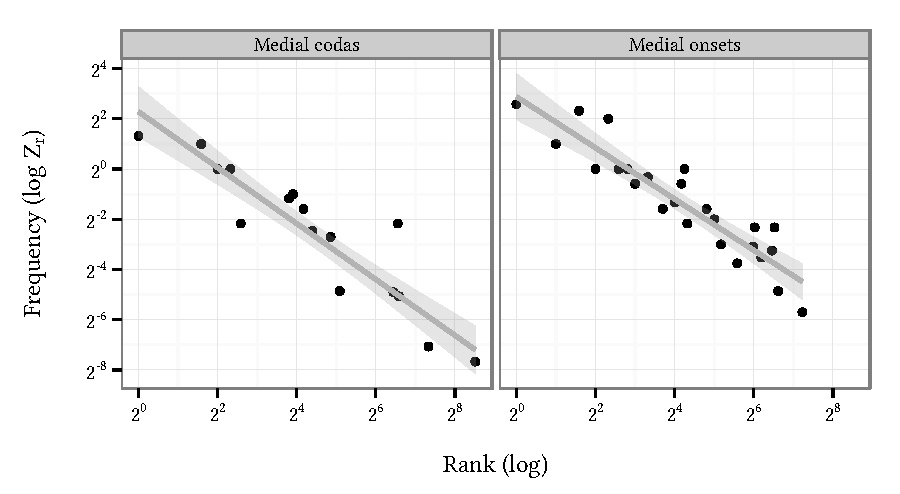
\includegraphics{co.pdf}
\caption{Medial coda and medial onset type frequencies in the lexical sample show a Zipfian distribution; frequencies have been smoothed using the $Z_r$ transform (see Appendix \ref{zr})}
\label{cao}
\end{figure}

\begin{example}[Simulation procedure]
\begin{tabular}{l l}
a. & Sample a medial coda according to the observed probabilities  \\
b. & Sample a medial onset according to the observed probabilities \\
c. & Apply the \emph{SPE} rules to the cluster formed by their concatenation \\
\end{tabular}
\end{example}

This procedure corresponds to the assumption that the medial cluster law the derived constraints impose the only structural restrictions on the cluster inventory.
Cluster frequencies in one simulated sample are shown in Figure \ref{sim}; points represent simulated frequencies and the line actual cluster frequencies.
As can be seen, the observed and simulated frequencies are quite similar (i.e., $R^2 = 0.712$; $p = 4.5$\e{-05}).
To summarize, the sparse cluster inventory, which \citeauthor{Pierrehumbert1994} takes as evidence for static constraints on syllable contact clusters, would result even if said static constraints do not exist.

\begin{figure}[t]
\centering
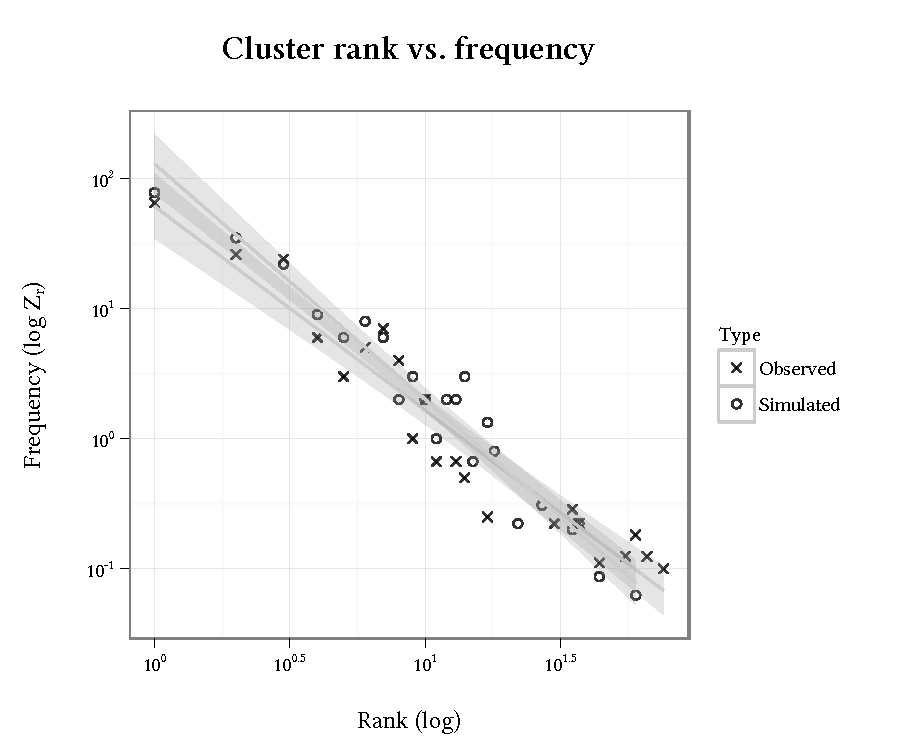
\includegraphics{sim.pdf}
\caption{A simulated cluster inventory closely matches the observed cluster frequencies (represented by the smoothing line); frequencies have been smoothed using the $Z_r$ transform (see Appendix \ref{zr})}
\label{sim}
\end{figure}

\section{Conclusions}

The foregoing results suggest that the only structural constraints on English syllable contact are derived from the phonological system: this study finds no evidence for static constraints.
The many other unattested clusters can only be understood as accidental gaps which are a consequence of the finite nature of the English lexicon.

%It is quite apparent that root-internal hetero-voiced obstruent clusters like [s.b] or [z.t] are also rare compared to clusters which are uniformly voiced or uniformly voiceless, as predicted the assimilation rule. Yet, \citet{Pierrehumbert1994} does not mention voice assimilation in her study of English syllable contact clusters. \citet[][74f.]{Hammond1999a} cites words like \emph{a}[b.s]\emph{inth} and \emph{a}[s.b]\emph{estos}, which contain hetero-voiced obstruent clusters, as evidence that the process does not apply root-internally, though few of his examples are in fact simplex according to CELEX.\footnote{The \textsc{Revised Alternation Condition} (RAC) proposed by \citeauthor{Kiparsky1973a} (\citeyear{Kiparsky1973a}:163, \citeyear{Kiparsky1982a}:152) blocks the application of obligatory neutralization processes like \textsc{Obstruent Voice Assimilation} in root-internal (i.e., non-derived) environments. Simply because there are exceptions in non-derived environments, \textsc{Obstruent Voice Assimilation} is always consistent with the RAC whether or not it actually applies in non-derived environments. This is due to the ``obligatory'' condition of the RAC. If the rule applies in non-derived environments, then it has lexical exceptions (e.g., \emph{a}[s.b]\emph{estos}) and is not obligatory and thus free from the RAC. On the other hand, if the rule is subject to the RAC, it only applies in derived environments, in which it is obligatory.}
% 
%The question is: does \textsc{Obstruent Voice Assimilation} contribute a meaningful characterization the English lexicon? More specifically, are hetero-voiced clusters underrepresented in a way that is unlikely under the hypothesis of free combination? To answer this question, the 720 clusters in which both the final coda consonant and initial onset consonant are obstruent are sorted into four bins, according to whether they are attested or not, and whether or not the conform to the derived constraint---both obstruents are either voiced or voiceless, like in \emph{hu}[z.b]\emph{and} or \emph{rha}[p.s]\emph{osdy}, respectively---or violate it, like the aforementioned \emph{a}[b.s]\emph{inth} and \emph{a}[s.b]\emph{estos}. 
